\documentclass[border=3pt]{standalone}
\usepackage{graphicx}
% source in fig/src/; images in fig/stages/ -> search both bases.
\graphicspath{{../stages/}{fig/stages/}{../}{./}}
\usepackage{tikz}
\usetikzlibrary{arrows.meta,calc,shadows.blur,positioning}
\definecolor{wacvblue}{rgb}{0.19,0.47,0.73}
\definecolor{amber}{rgb}{0.90,0.56,0.09}
\definecolor{slate}{rgb}{0.28,0.33,0.41}
% inline glyphs (drawn -> no font dependency), matching the teaser
\newcommand{\playicon}{\raisebox{-0.1ex}{\tikz[baseline]{\fill[white] (0,-0.5mm)--(0,1.5mm)--(1.6mm,0.5mm)--cycle;}}}
\newcommand{\pulseicon}{\raisebox{0.1ex}{\tikz[baseline]{\draw[white,line width=0.45pt,line cap=round,line join=round]
   (0,0.3mm)--(0.6mm,0.3mm)--(1.1mm,1.5mm)--(1.7mm,-0.9mm)--(2.3mm,0.5mm)--(2.9mm,0.5mm);}}}
\begin{document}
\begin{tikzpicture}[
  softshadow/.style={blur shadow={shadow blur steps=6, shadow xshift=0pt,
                     shadow yshift=-0.6pt, shadow opacity=26, shadow blur radius=1.0pt}},
  frame/.style={draw=wacvblue!70, line width=0.9pt, rounded corners=1.5pt,
                inner sep=0pt, softshadow},
  pill/.style={rounded corners=2.5pt, inner sep=2.8pt, font=\bfseries\footnotesize,
               text=white, softshadow},
]
  % ---------- EEG panel (bottom), amber-bordered ----------
  \node[anchor=south west, inner sep=0, draw=amber!75, line width=1pt, rounded corners=2pt]
       (eeg) at (0,0) {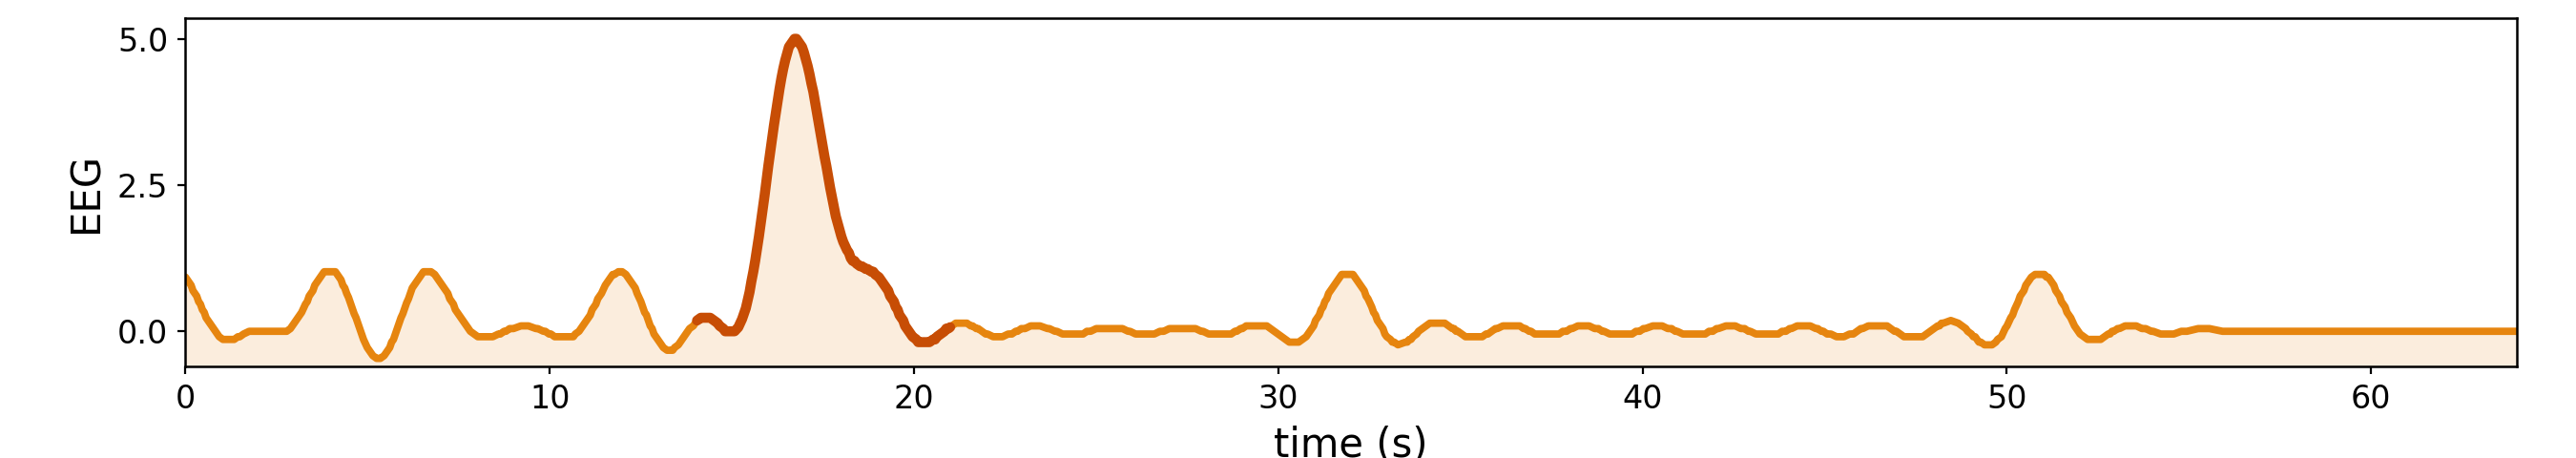
\includegraphics[width=13cm]{b_eeg_bold.png}};
  % data-area x anchors (measured on b_eeg_bold: t=0 -> 0.0726 W, t=64 -> 0.9763 W)
  \coordinate (dl) at ($(eeg.south west)!0.0726!(eeg.south east)$);
  \coordinate (dr) at ($(eeg.south west)!0.9763!(eeg.south east)$);
  % ictal-window highlight [15,20] s + peak callout (peak ~17 s near plot top).
  % Label/arrow use pure-calc (partway on the north edge + shift): an inline $...$
  % calc on the LEFT of |- does not parse inside a node/coordinate `at`.
  \fill[amber, opacity=0.18] ($(dl)!{15/64}!(dr)$ |- eeg.south)
                             rectangle ($(dl)!{20/64}!(dr)$ |- eeg.north);
  \node[font=\scriptsize, text=amber!55!black, anchor=south west] (ilab)
       at ($(eeg.north west)!0.4397!(eeg.north east)+(0,-6.5mm)$) {ictal discharge};
  \draw[amber!65!black, -{Stealth[length=1.5mm]}, line width=0.55pt]
       (ilab.west) to[out=180,in=-35] ($(eeg.north west)!0.3126!(eeg.north east)+(0,-1.7mm)$);
  % EEG tab (over the empty top-left of the plot, right of the y-axis)
  \node[pill, fill=amber!82!black, anchor=north west]
       at ([xshift=1mm,yshift=-1mm]$(dl |- eeg.north)$) {\pulseicon~EEG};
  % ---------- faint quarter guides linking timeline to the frames ----------
  \foreach \f in {0.25,0.5,0.75}{
    \draw[black!16, dashed, line width=0.5pt, dash pattern=on 1.2pt off 1.2pt]
         ($(dl)!\f!(dr)$ |- eeg.north) -- ($(dl)!\f!(dr) + (0,1.78)$);
  }
  % ---------- video frame strip (top), aligned above the EEG time axis ----------
  \foreach \k/\n in {0/1,1/2,2/3,3/4}{
    \node[frame, anchor=south] (f\k)
      at ($(dl)!{(\k+0.5)/4}!(dr) + (0,2.81)$)
      {\includegraphics[width=2.75cm]{b_v\n_enh.png}};
  }
  % VIDEO tab, top-left above the strip
  \node[pill, fill=wacvblue!85, anchor=south west] at ([yshift=0.8mm]f0.north west) {\playicon~VIDEO};
  % subtle "sampled across the clip" hint on the right of the strip
  \node[font=\scriptsize\itshape, text=slate, anchor=south east]
       at ([yshift=0.8mm]f3.north east) {sampled across the $\sim$64\,s clip};
\end{tikzpicture}
\end{document}
